\chapter{Previous work} \label{sec:previous_work}

\section{Food localization}

circle detection if we make the asumption that the food is in a plate / bowl: 2.2 + 6.3 + \cite{Dehais2015}

color segmentation vs edge segmentation: 11.1 (very limited test)

DCNN: 3.2 + * + 9.1

\section{Food recognition}

Food recognition

Using SVM:

Local using BOW: 3.3
gloabal feature:
Color and texture description: 
Spatial pyramid:

Mix of several features:

DCNN: *

\section{Food intake}

FoodLog \footnote{\url{http://www.foodlog.jp}} is a website that enables the user to upload pictures of its daily meals to be archived and processed. The goal of this application is to assist the user to keep notes of their meals and balance the nutritional values coming from different kinds of food.

In \cite{Kitamura2008}, the images containing food items are identified by exploiting features related to the HSV and RGB colour domains, as well as the shape of the plate. A SVM classifier is trained to detect food images. More specifically, the images are divided in 300 blocks and each block is classified as \enquote{non-food} (discarded block) or one of the nutritional categories described in the \enquote{MyPyramid} model \footnote{\url{http://www.mypyramid.gov}}.

MyPyramid \cite{MyPyramid} was designed by the United State Departement of Agriculture \textit{USDA} in 2005 and was replaced in 2011 by \enquote{MyPlate} \footnote{\url{http://www.choosemyplate.gov}} \cite{MyPlate}. This dietary model is composed of 5 kinds of food: grains, vegetable, meals and beans, milk and fruit. For each group, a recommended intake per day is associated, Fig. \ref{fig:my_pyramid}. Quantity is categorized by \enquote{servings} \textit{SV}, making it simpler to compute and keep log.

In \cite{Aizawa2013} the Support Vector Machine is replaced by a Bayesian Framework \textit{BF}.
The BF is based on the Gaussian Naive Bayesian (suppose independence between every pair of features and the distribution of each feature is assumed to be Gaussian). The BF takes into account the estimation using color moments and Bag-Of-Feature of SIFT, the prior distribution and the mealtime category (breakfast, lunch and dinner).

\begin{figure}
    \centering
    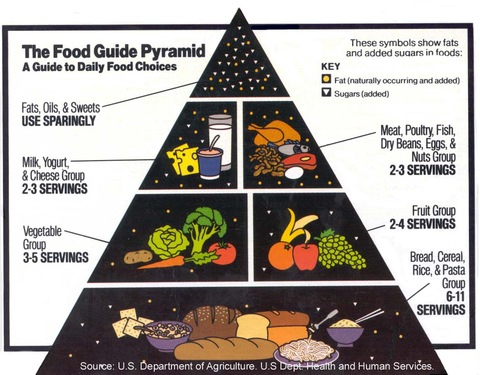
\includegraphics[scale=0.8]{img/my_pyramid.jpg}
    \caption{USDA MyPyramid original logo}
    \label{fig:my_pyramid}
\end{figure}

Food Cam